% !TeX root = ../praktikum.tex
% !TeX encoding = UTF-8
% !Tex spellcheck = de_DE

In diesem Abschnitt wurde die recht zeitaufwändige Justage der Lasereinheit durchgeführt, mit dem Ziel, den Laserstrahl in eine Glasfaser einzukoppeln. Der Vorteil einer Faser ist, dass der anschließende Aufbau zur Durchführung der Fouriermessungen an beliebig anderer Stelle im Labor errichtet werden kann. 
Der Faserkopplungsaufbau (siehe Abbildung \ref{fig:lasereinheit}) befand sich in bereits aufgebautem Zustand auf einer eigenen Platte und wurde lediglich optimiert. Für die Durchführung des Versuchs wurde ein temperaturgesteuerter cw-Diodenlaser \footnote{Modell  \textit{LD: Mitsubishi ML101J27} mit einer maximalen Ausgangsleistung von \unit[35]{mW} verwendet. Betrieben wurde der Laser mit 90,3 mA bei $18^\circ C$.} mit einer Wellenlänge von \unit[660]{nm}.

\begin{figure}[h]
	\centering
	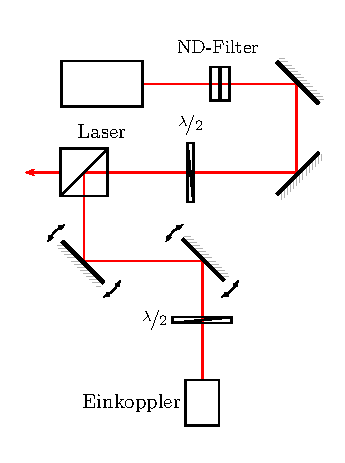
\includegraphics[width=0.5\linewidth]{graphs/versuchsaufbau/lasereinheit.pdf}
	\caption[Schematischer Aufbau Lasereinheit]{
		Schematischer Strahlungsaufbau zwischen Laser und Fasereinkopplung. Nach dem Verlassen des Lasers wird die Lichtintensität aus Sicherheitsgründen mit Hilfe eines ND-Filters reduziert. Mit Hilfe der darauf folgenden Spiegel wurde der Strahlenverlauf feinjustiert. Der Strahlteiler dient dazu, dass je zwei Versuchsaufbauten Licht erhalten. Mit Hilfe der sich davor befindlichen $\nicefrac{\lambda}{2}$- Platte die Intensität des Laserstrahls so eingestellt werden, dass beide Versuchsaufbauten ausreichend Lichtleistung erhalten. Der zweite Strahl nach dem Strahlteiler wird nicht weiter betrachtet.
	}
	\label{fig:lasereinheit}
\end{figure}

 Zur Regulierung der Intensität wurde die Eigenschaft der Polarisation des Lichts ausgenutzt, welche anschaulich als \textit{Schwingungsebene} einer Lichtwelle beschrieben werden kann. Der Laserstrahl durchläuft eine $\nicefrac{\lambda}{2}$-Platte; dabei handelt es sich um eine doppelbrechende Platte, welche den beiden entstehenden Teilwellen einen Gangunterschied erteilt, der gleich der Hälfte der Bezugswellenlänge $\lambda$ ist. In Diagonalstellung wird die Polarisation des Lichts gedreht. Letzterer Effekt wurde hier genutzt, da so in Kombination mit dem Strahlteiler hinter der $\nicefrac{\lambda}{2}$-Platte die Menge des anschließend verwendeten Lichts wie folgt reguliert werden konnte. Der Strahlteiler ist für eine der beiden Polarisationsebenen durchlässig, für die Andere reflektierend. Durch Drehung der $\nicefrac{\lambda}{2}$-Platte wurde die Polarisation des Lichts beeinflusst. So konnte beeinflusst werden, wie hoch der Anteil des Lichts mit der Polarisation ist, welche durch den Strahlteiler zur Glasfaser gelenkt wurde. Auch direkt vor der Fasereinkopplung spielt die Polarisation eine Rolle, da die lichtleitende Faser für eine bestimmte Polarisation die höchste Effizienz aufweist. Aus diesem Grund befindet sich im Aufbau eine weitere $\nicefrac{\lambda}{2}$-Platte unmittelbar vor der Fasereinkopplung.\\

Mit der Glasfaser wird das Licht anschließend zum eigentlichen Experiment geleitet. Dabei wird ausgenutzt, dass Licht, welches auf einen Brechzahlsprung trifft, total reflektiert wird, wenn es unter einem sehr kleinen Winkel auftrifft. Aus diesem Grund müssen die Lichtstrahlen unter möglichst geringem Winkel in die Glasfaser eintreten. So muss für die Einkopplung also sowohl die sehr dünne Faser getroffen werden, als auch der Eintrittswinkel möglichst genau angepasst werden.

Als Hilfestellung für diese Einkopplung des Lichts in die Faser wurde ein Laserpointer an dem noch freien Ende der Faser angebracht und vor dem Einkoppler mit Hilfe der Spiegel eine optimale Überlagerung der beiden Signale eingestellt. So wurde das Axiom der Strahlenumkehr der geometrischen Optik genutzt, um den Laserstrahl unter dem korrekten Winkel und Ort einzukoppeln. Dies gelingt recht schnell, da jedoch sowohl die Faser als auch der Laserstrahl eine räumliche Ausdehnung haben, erhält man anfangs häufig sehr geringe Intensitäten. Deswegen wurde der Laserpointer entfernt und die Intensität per Auge beobachtet und verbessert. Da aufgrund der relativ hohen Lichtintensitätsdichten die Intensitätsschwankungen  nur schwer zu erkennen sind, wurde anschließend die Intensität des aus der Faser austretenden Lichtes mit einem Powermeter gemessen, um dessen Leistung anhand der Feinjustierung über die Spiegel weiter zu optimieren. Das Powermeter, welches an ein Oszilloskop angeschlossen wurde, konnte auch schnelle Änderungen der gemessenen Lichtleistung besser sichtbar machen.

Der Winkel, unter welchem der Laserstrahl auf den Einkoppler traf, wurde mittels des sogenannten \textit{Walkens} optimiert. Hierbei wird an den beiden letzten Spiegeln vor dem Einkoppler gleichzeitig an den Schrauben jeweils einer Achse, beispielsweise der Vertikalen, entgegengesetzt gedreht. Bei dieser Technik wird der Strahl über den ersten Spiegel beispielsweise nach oben gelenkt und über den Zweiten nach unten. Die Position des Eintreffenden Lichtstrahls bleibt also erhalten, während der Einfallswinkel variiert werden kann. So lässt sich letztlich der Strahl genau in die Faser einkoppeln.

Nachdem hierfür ein Optimum auf dem Oszilloskop möglichst genau eingestellt wurde, wurde die Faser unter Beobachtung des Signals auf dem Oszilloskop verbogen und mit Hilfe eines Heißluftföhns erhitzt und gleichzeitig die $\nicefrac{\lambda}{2}$-Platte vor der Einkopplung in ihrer Halterung gedreht. Steht die $\nicefrac{\lambda}{2}$-Platte optimal, so ist die Polarisation erreicht, für welche die Glasfaser die höchste Transmission aufweist. Dies zeigt sich daran, dass das beobachtbare Signal auf dem Oszilloskop unter Verbiegen und Erhitzen die geringsten Schwankungen aufweist. \\
Bei dem hier gefundenen Optimum der Fasereinkopplung wurde mit einem Powermeter vor der Einkopplung eine Spannung von \unit[420]{mV} gemessen und hinter der Auskopplung eine Spannung von \unit[244]{mV}. Dies entspricht einer Effizienz von 42\%. 

